
\section{ Geometry}
\begin{frame}
    \frametitle{The School of Athens by Raphel}
    
    \begin{center}
        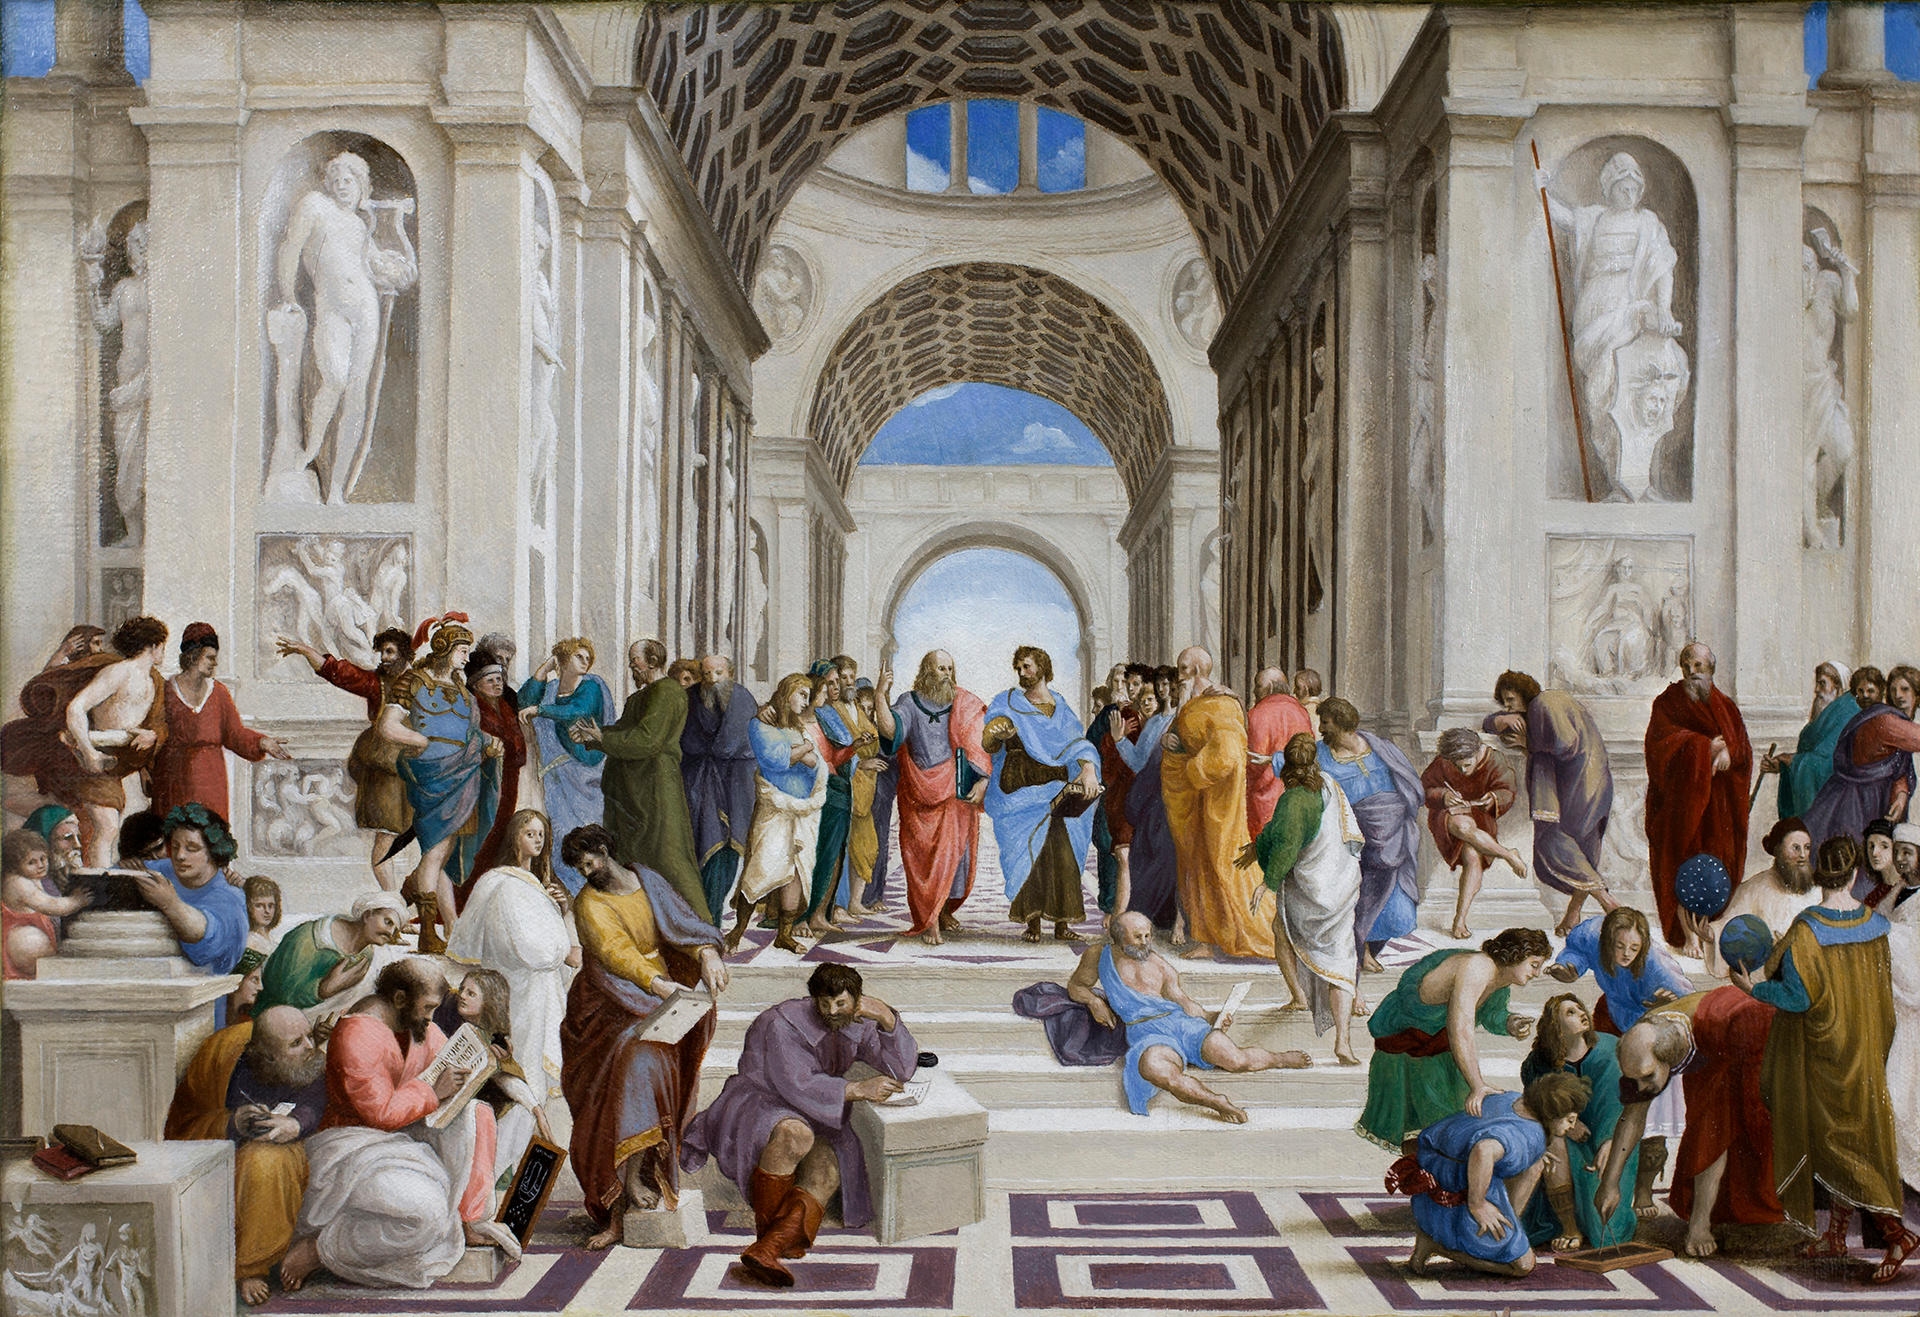
\includegraphics[width=0.9\textwidth]{intro/the_school_of_athens.jpg} % Add an appropriate image to illustrate supplementary and complementary angles
    \end{center}
\end{frame}

\begin{frame}{What is Geometry?}
    \begin{itemize}
        \item Branch of mathematics studying shapes, sizes, and spatial relationships.
        \item Derived from Greek: \textit{"geo"} (earth) + \textit{"metron"} (measure).
        \item Originally focused on measuring the earth, now much broader.
    \end{itemize}
\end{frame}

\begin{frame}{Key Concepts in Geometry}
    \begin{itemize}
        \item \textbf{Points, Lines, and Angles}: Basic building blocks.
        \item \textbf{Shapes and Figures}: Circles, triangles, polygons.
        \item \textbf{Solids}: 3D objects like cubes, spheres, pyramids.
        \item \textbf{Theorems and Proofs}: Logical reasoning based on axioms and postulates.
    \end{itemize}
\end{frame}

\begin{frame}{Why Learning Geometry is Important in ML}
    \begin{itemize}
        \item \textbf{Understanding Data:} ML operates in high-dimensional spaces, where geometry helps analyze structure and relationships.
        \item \textbf{Feature Engineering:} Transformations (rotations, scaling, projections) improve model performance.
        \item \textbf{Distance Metrics:} Algorithms rely on distances (Euclidean, cosine, Manhattan) for clustering and classification.
        \item \textbf{Optimization:} Gradient descent follows geometric paths to minimize loss functions.
        \item \textbf{Manifold Learning:} Real-world data often lies on curved manifolds, requiring non-Euclidean methods (e.g., t-SNE, UMAP).
        \item \textbf{Deep Learning:} CNNs use geometric transformations; GNNs handle graph structures.
        \item \textbf{Model Interpretability:} Decision boundaries (e.g., SVMs) are geometric constructs that explain model behavior.
    \end{itemize}
    \end{frame}


\begin{frame}{Definition of Percentage}
    \begin{itemize}
        \item A \textbf{percentage} is a way of expressing a number as a fraction of 100.
        \item The formula to calculate a percentage is:
    \[
        \text{Percentage} = \left( \frac{\text{Part}}{\text{Whole}} \right) \times 100
    \]
        \item Example: If you score 45 out of 60 on a test, the percentage is:
    \[
        \left( \frac{45}{60} \right) \times 100 = 75\%
    \]
    \end{itemize}
\end{frame}

\begin{frame}
    \frametitle{Ratio vs Rate}
    \begin{figure}[h]    
        \begin{minipage}[b]{0.5\textwidth}
        \centering
        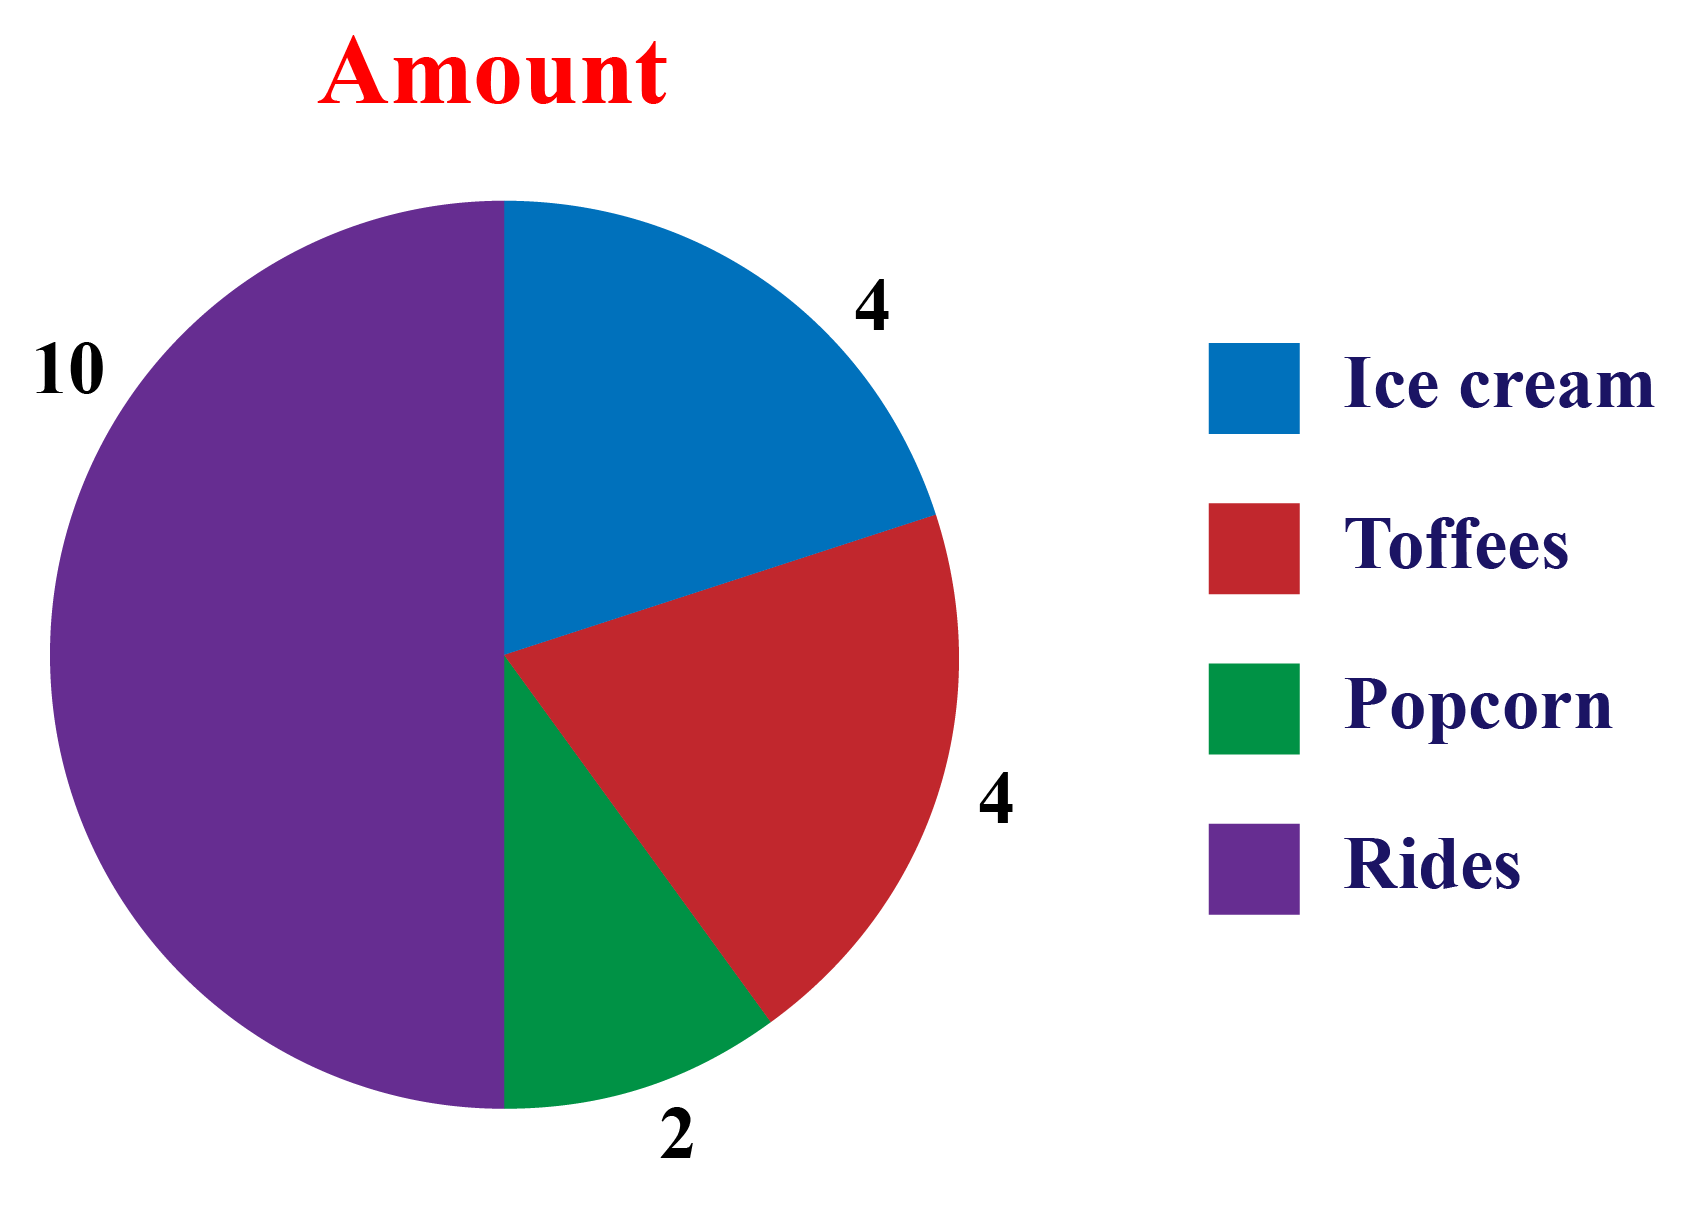
\includegraphics[scale=0.2]{intro/ratio.png}
        \caption{ratio}
    \end{minipage}
    \begin{minipage}[b]{0.4\textwidth}
        \centering
        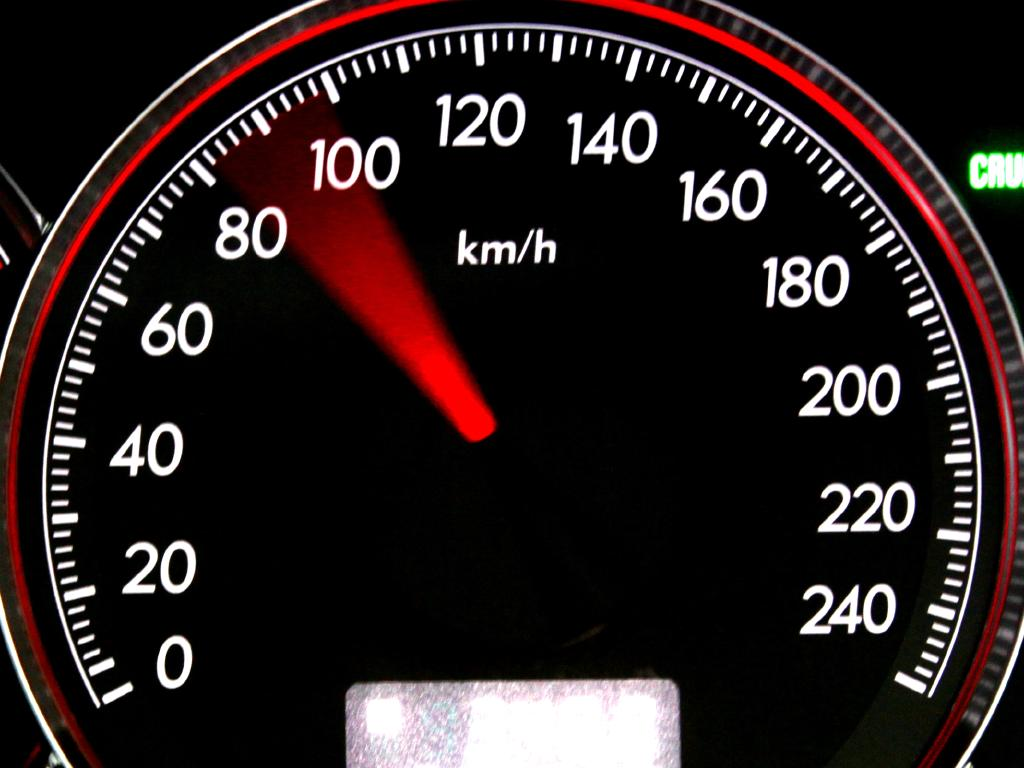
\includegraphics[scale=0.5]{intro/rate.jpeg}
        \caption{rate}
    \end{minipage}
\end{figure}
\end{frame}

\begin{frame}{Key Distinction: Ratio vs Rate}
    \begin{columns}[T] % Split into two columns
        \column{0.5\textwidth}
        \centering
        \textbf{Ratio}
        \begin{itemize}
            \item \textbf{Definition:} Comparison of two similar units.
            \item \textbf{Units:} Unitless (dimensionless).
            \item \textbf{Form:} Written as \( a:b \), \( \frac{a}{b} \), or "a to b".
            \item \textbf{Example:} Boys to girls in a classroom is \( 2:3 \).
            \item \textbf{Key Feature:} Static relationships.
        \end{itemize}

        \column{0.5\textwidth}
        \centering
        \textbf{Rate}
        \begin{itemize}
            \item \textbf{Definition:} Comparison of two different units.
            \item \textbf{Units:} Includes units (e.g., miles per hour).
            \item \textbf{Form:} Written as \( \frac{a \, \text{unit}_1}{b \, \text{unit}_2} \) or "a per b".
            \item \textbf{Example:} A car travels \( 60 \, \text{mph} \).
            \item \textbf{Key Feature:} Dynamic relationships (e.g., over time or space).
        \end{itemize}
    \end{columns}
\end{frame}


\begin{frame}
    \frametitle{Proportional Relationship}

    \begin{block}{Definition}
        A proportional relationship is a relationship between two quantities where the ratio between them remains constant. 
        If two variables are proportional, it means they can be expressed in the form:
        \[ y = kx \]
        where $ k $ is the constant of proportionality and it can be an integer or a fraction or an irrational number.
    \end{block}
\end{frame}

\begin{frame}
    \frametitle{Proportionality Problem: Mixing Chemicals}

    \begin{block}{Problem}
        A person mixes $15 ml$ of bleach with $3.75 L$ of water for sanitizing solution for a daycare. What are the possible combinations 
    \end{block}

    \begin{itemize}
        \item \textbf{A.} 12 mL bleach and 3L water
        \item \textbf{B.} 6 mL bleach and 1.5L water
        \item \textbf{C.} 3 mL leach and 0.75L water
        \item \textbf{D.} 20 mL bleach and 5.5L water
    \end{itemize}
    \begin{block}{Problem}
        Is the area of square is propotional to side length ?
    \end{block}
\end{frame}

\begin{frame}{Proportionality vs. Linearity}
    \begin{itemize}
        \item A \textbf{proportional relationship} always passes through the origin \((0, 0)\).
        \item The general form of a proportional relationship is:
        \[
        y = kx
        \]
        where \(k\) is the constant of proportionality.
        
        \item A \textbf{linear relationship} can pass through any point, not necessarily the origin.
        \item The general form of a linear relationship is:
        \[
        y = mx + b
        \]
        where \(m\) is the slope and \(b\) is the y-intercept.
        
        \item Key Difference:
        \begin{itemize}
            \item In a proportional relationship, \(b = 0\), so the line always passes through \((0, 0)\).
            \item In a linear relationship, \(b\) can be any value, so the line does not need to pass through the origin.
        \end{itemize}
    \end{itemize}
\end{frame}


\begin{frame}{Main Types of Geometry}
    \begin{itemize}
        \item \textbf{Euclidean Geometry}: Deals with flat, 2D spaces.
        \item \textbf{Non-Euclidean Geometry}: Studies curved spaces (spherical, hyperbolic).
        \item \textbf{Analytic Geometry}: Combines algebra and geometry using coordinates.
        \item \textbf{Differential Geometry}: Uses calculus to study curves and surfaces.
    \end{itemize}
\end{frame}

\begin{frame}{Applications of Geometry}
    \begin{itemize}
        \item Essential in fields like architecture, physics, engineering.
        \item Used in navigation, astronomy, and computer graphics.
        \item Provides tools to understand spatial relationships in various disciplines.
    \end{itemize}
\end{frame}

\subsection{Eucledian Geometry} 

\begin{frame}
    \frametitle{Geometry Terminology}
    
    \begin{center}
        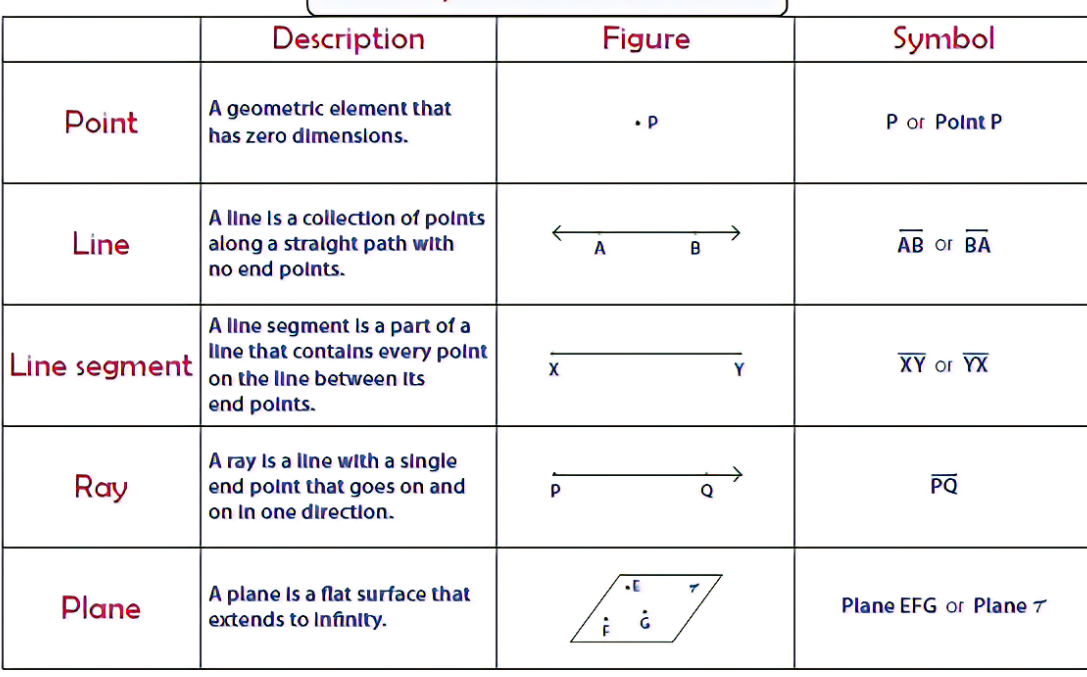
\includegraphics[width=0.8\textwidth]{intro/geometry.png} % Add an appropriate image to illustrate supplementary and complementary angles
    \end{center}
\end{frame}
\begin{frame}
    \frametitle{Geometry Terminology: Coplanar \& Colinear}
    \begin{center}
        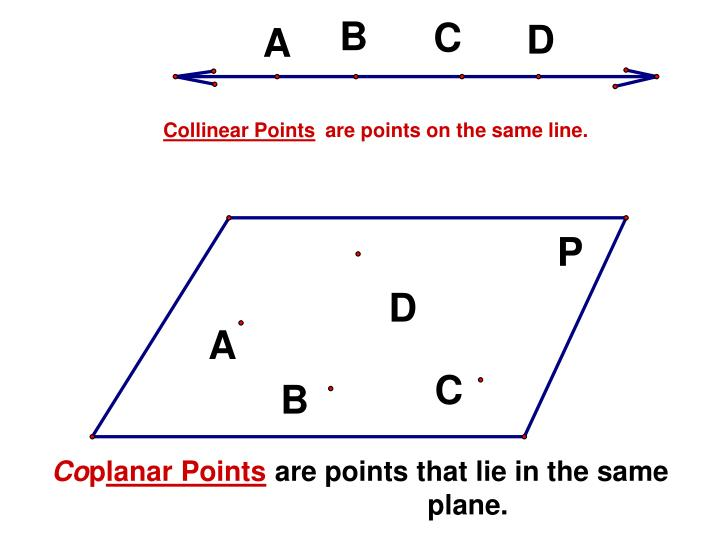
\includegraphics[width=0.8\textwidth]{intro/coplanar.jpg} % Add an appropriate image to illustrate supplementary and complementary angles
    \end{center}
\end{frame}

\begin{frame}
    \frametitle{Geometry Terminology: Dimensions}
    \begin{center}
        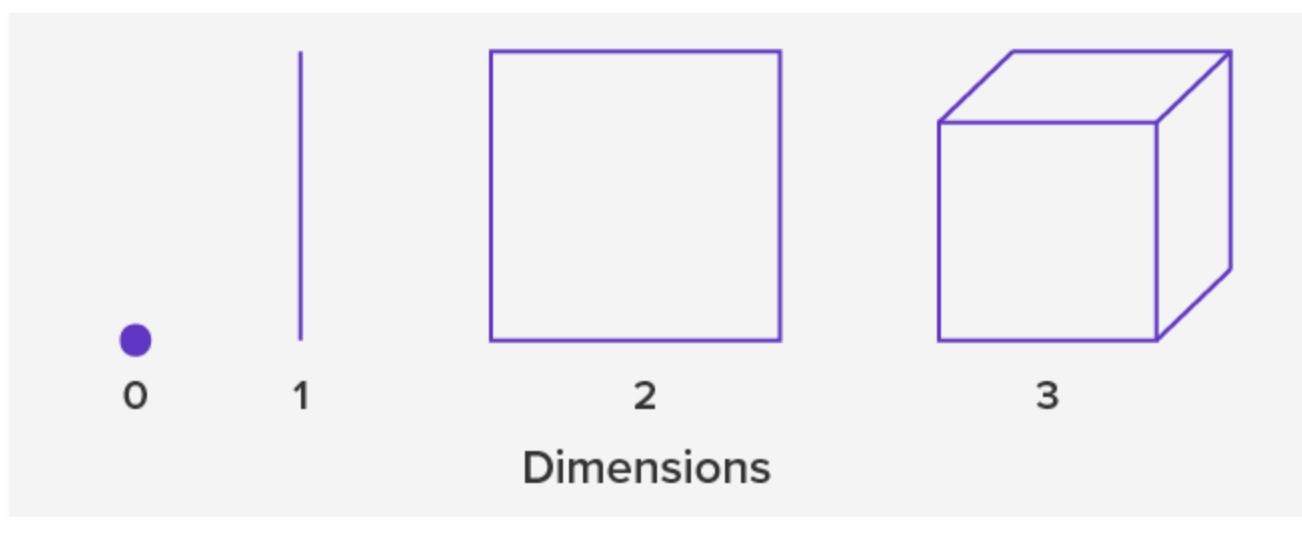
\includegraphics[width=0.8\textwidth]{intro/dimensions.jpeg} % Add an appropriate image to illustrate supplementary and complementary angles
    \end{center}
\end{frame}

\begin{frame}{Parallel \& Perpendicular Lines}
    \begin{block}{Parallel}
      Two lines are said to be \textbf{parallel} if they never intersect, no matter how far they are extended, and remain the same distance apart at all points.
    \end{block}
    \begin{block}{Perpendicular}
        Two lines are said to be \textbf{perpendicular} if they intersect at a right angle (90 degrees).
    \end{block}
  \end{frame}


  \begin{frame}
    \frametitle{Parallel \& Perpendicular Lines}
    \begin{center}
        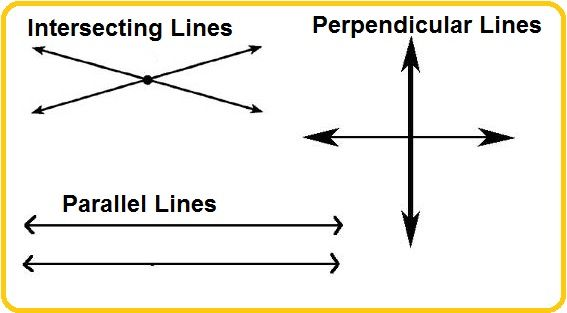
\includegraphics[width=0.8\textwidth]{intro/parallel_perpendicular.jpg} % Add an appropriate image to illustrate supplementary and complementary angles
    \end{center}
\end{frame}




\begin{frame}{Angles}
    \begin{itemize}
        \item \textbf{Angle}: Formed by two rays with a common endpoint.
        \item \textbf{Acute Angle}: Less than 90°.
        \item \textbf{Right Angle}: Exactly 90°.
        \item \textbf{Obtuse Angle}: Greater than 90° but less than 180°.
        \item \textbf{Straight Angle}: Exactly 180°.
    \end{itemize}
\end{frame}

\begin{frame}{Shapes and Figures}
    \begin{itemize}
        \item \textbf{Polygon}: A closed figure formed by line segments.
        \item \textbf{Triangle}: A polygon with three sides.
        \begin{itemize}
            \item \textbf{Equilateral Triangle}: All sides and angles are equal.
            \item \textbf{Isosceles Triangle}: Two sides and angles are equal.
            \item \textbf{Scalene Triangle}: All sides and angles are different.
        \end{itemize}
        \item \textbf{Quadrilateral}: A polygon with four sides (e.g., square, rectangle).
        \item \textbf{Circle}: A set of points equidistant from the center.
    \end{itemize}
\end{frame}

\begin{frame}{Properties of Shapes}
    \begin{itemize}
        \item \textbf{Perimeter}: Total distance around a shape.
        \item \textbf{Area}: The measure of space inside a two-dimensional shape.
        \item \textbf{Volume}: The measure of space inside a three-dimensional object.
    \end{itemize}
\end{frame}

\begin{frame}{Transformations}
    \begin{itemize}
        \item \textbf{Translation}: Moving a shape without rotating or flipping it.
        \item \textbf{Rotation}: Turning a shape around a fixed point.
        \item \textbf{Reflection}: Flipping a shape over a line to create a mirror image.
        \item \textbf{Dilation}: Resizing a shape while maintaining its proportions.
    \end{itemize}
\end{frame}

\begin{frame}
    \frametitle{Parallel Lines}
    
    \begin{itemize}
        \item \textbf{Definition:} Two or more lines that are always the same distance apart and never meet, no matter how far they are extended.
        \item They run in the same direction and have the same slope.
        \item Example: Think of train tracks running side by side—they never cross each other.
    \end{itemize}
    
    \begin{center}
        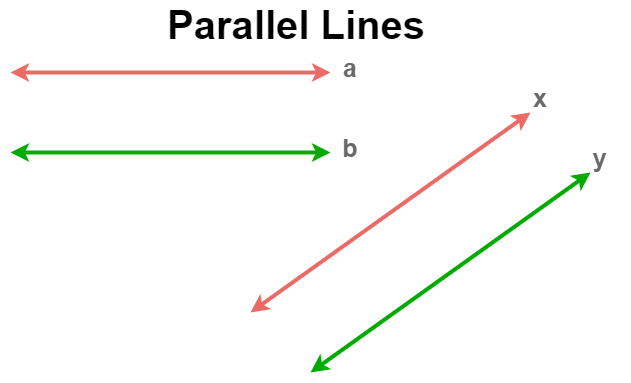
\includegraphics[width=0.5\textwidth]{intro/Parallellines.png} % Add an appropriate image to illustrate parallel lines
    \end{center}

\end{frame}
\begin{frame}
    \frametitle{Angles}
\end{frame}

\begin{frame}
    \frametitle{Supplementary and Complementary Angles}
       
    \begin{center}
        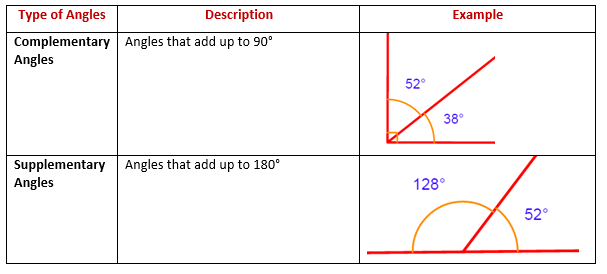
\includegraphics[width=0.9\textwidth]{intro/complementary_supplementary_angles.png} % Add an appropriate image to illustrate supplementary and complementary angles
    \end{center}

\end{frame}

\begin{frame}
    \frametitle{Problem 1}
    
    \begin{center}
        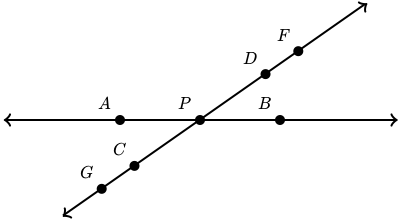
\includegraphics[width=0.9\textwidth]{intro/supplementary_angles.png} % Add an appropriate image to illustrate supplementary and complementary angles
    \end{center}

\end{frame} 

\begin{frame}
    \frametitle{Vertical Angles}
    \begin{block}{}
        Vertical angles, also known as opposite angles, are the angles formed when two lines intersect
    \end{block}
    \begin{center}
        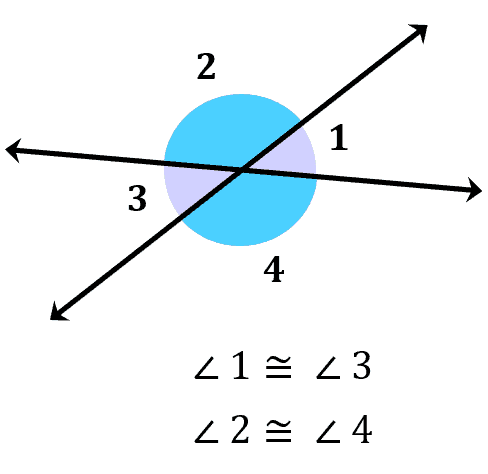
\includegraphics[width=0.5\textwidth]{intro/vertical_angles_1.png} % Add an appropriate image to illustrate supplementary and complementary angles
    \end{center}

\end{frame}


\begin{frame}
    \frametitle{Problem 2: Vertical Angles}
\begin{center}
    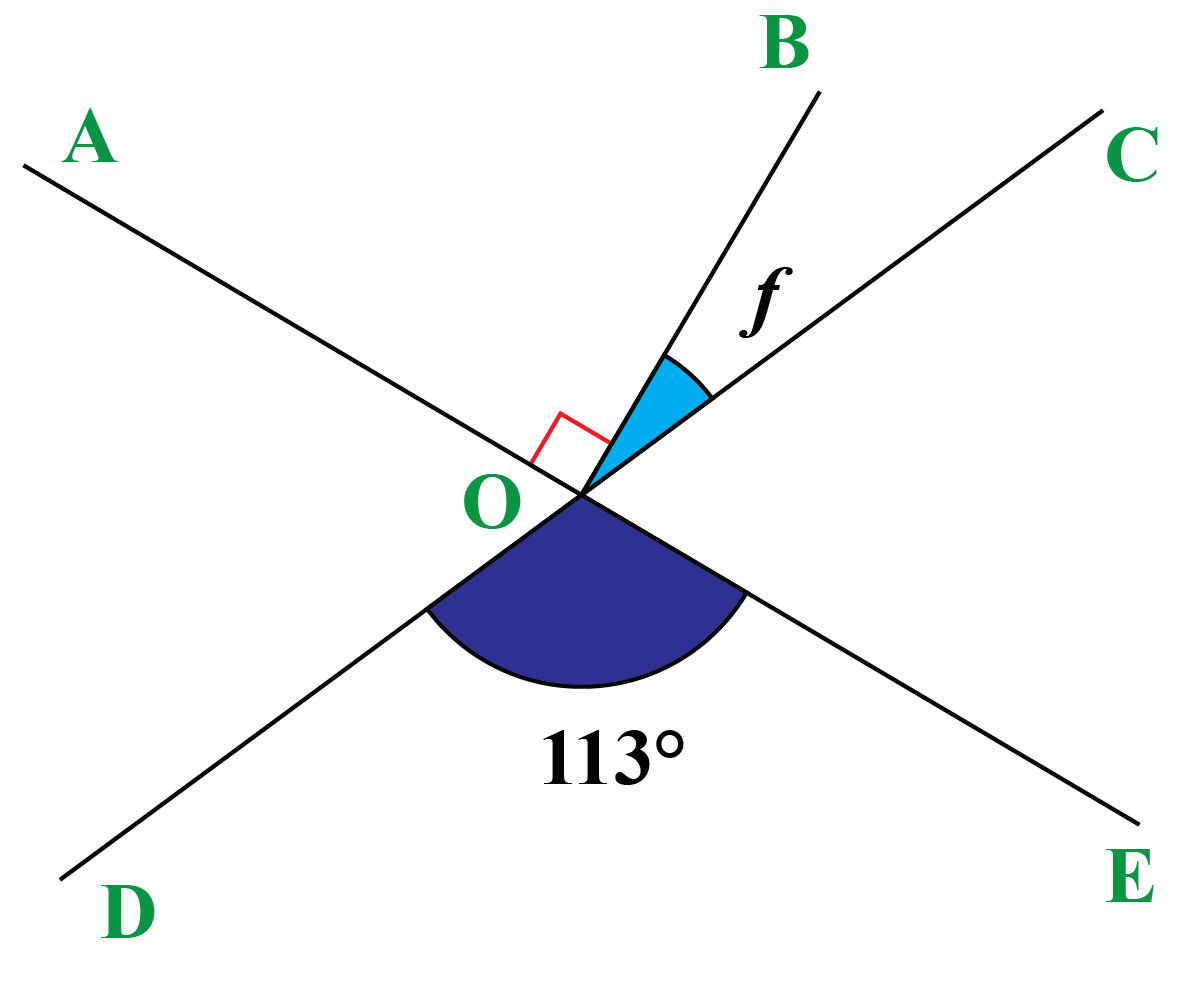
\includegraphics[width=0.5\textwidth]{intro/vertical_angles_2.png} % Add an appropriate image to illustrate supplementary and complementary angles
\end{center}
\end{frame}


\begin{frame}{Transversal \& Parallel Lines}
    A \textbf{transversal line} is a line that crosses or intersects two or more other lines at different points
    \begin{figure}[h]    
        \begin{minipage}[b]{0.4\textwidth}
        \centering
        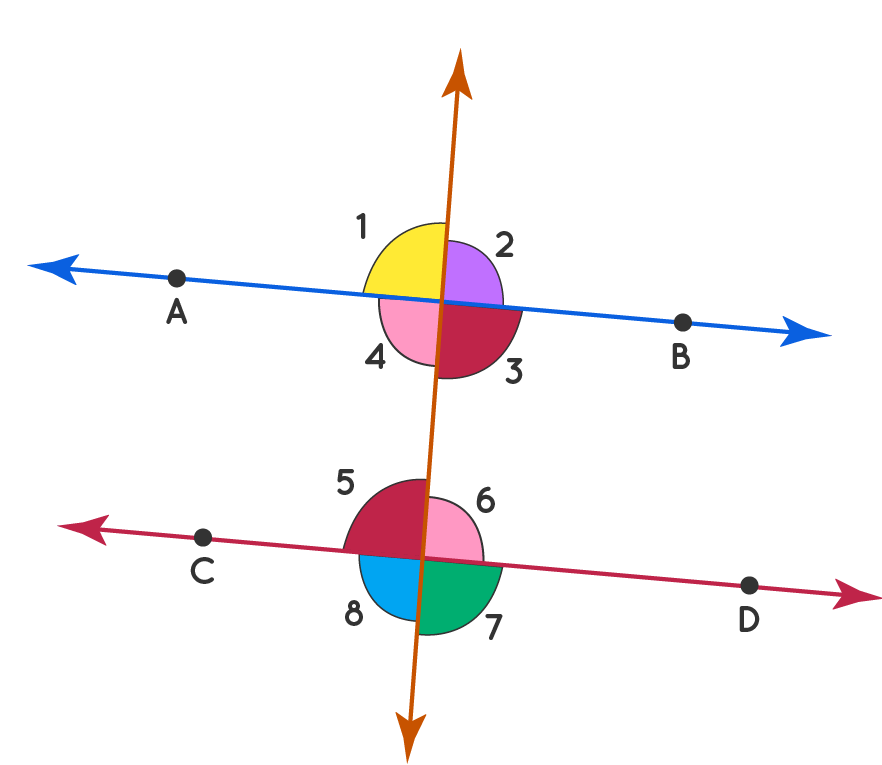
\includegraphics[scale=0.15]{intro/alternate_interior_angles.png}
        \caption{alternate interior angles}
    \end{minipage}
    \begin{minipage}[b]{0.4\textwidth}
        \centering
        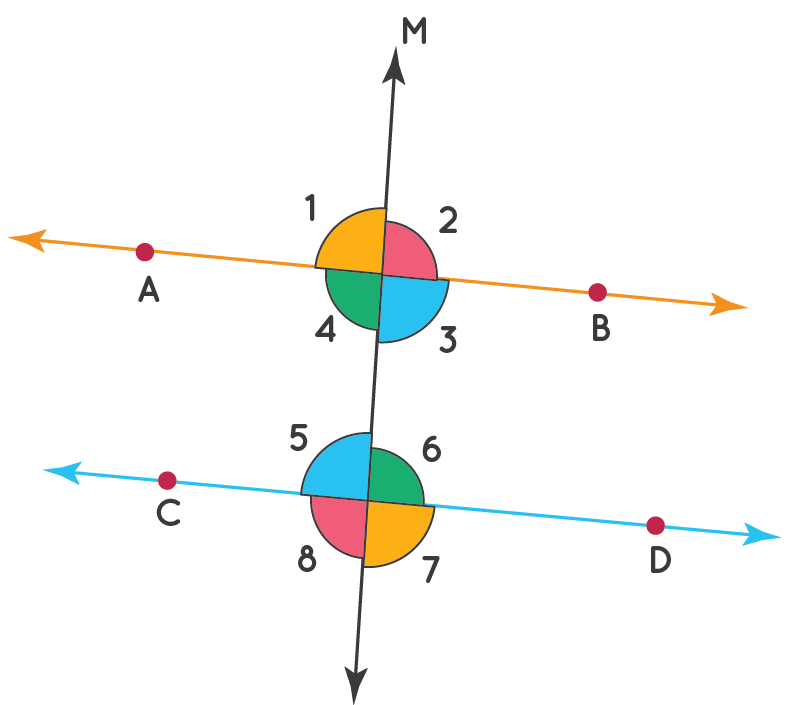
\includegraphics[scale=0.15]{intro/alternate_exterior_angles.png}
        \caption{alternate exterior angles}
    \end{minipage}
\end{figure}
    
\end{frame}




\begin{frame}
    \frametitle{Altitudes, Medians and Centroid} 

    \begin{figure}[h]    
        \begin{minipage}[b]{0.4\textwidth}
        \centering
        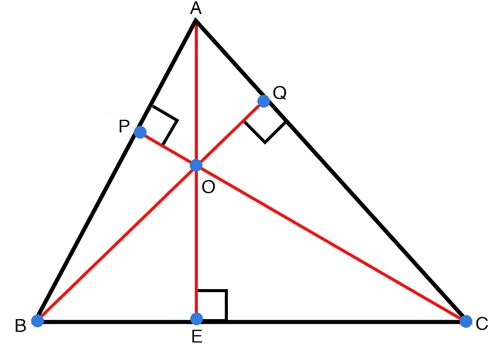
\includegraphics[scale=0.25]{intro/altitudes.jpeg}
        \caption{altitudes}
    \end{minipage}
    \begin{minipage}[b]{0.4\textwidth}
        \centering
        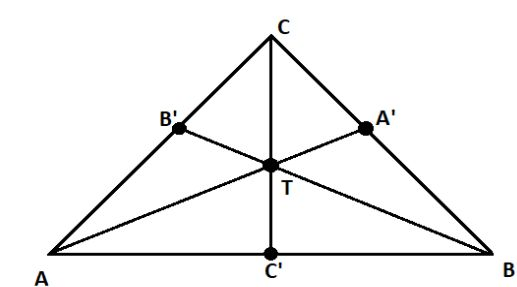
\includegraphics[scale=0.25]{intro/medians.jpeg}
        \caption{medians}
    \end{minipage}
\end{figure}
\end{frame}

\begin{frame}
    \frametitle{Exterior Angle Property}
    \begin{center}
        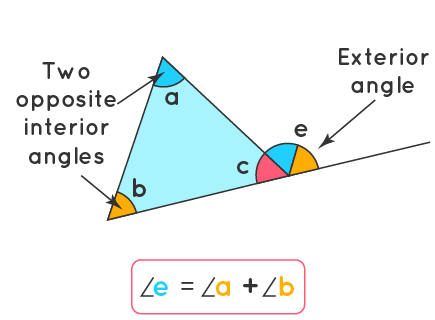
\includegraphics[width=0.5\textwidth]{intro/exterior_angle.png} 
    \end{center}
\end{frame}

\begin{frame}
    \frametitle{Angles of a Triangle Measure to $180^\circ$}
    \begin{center}
        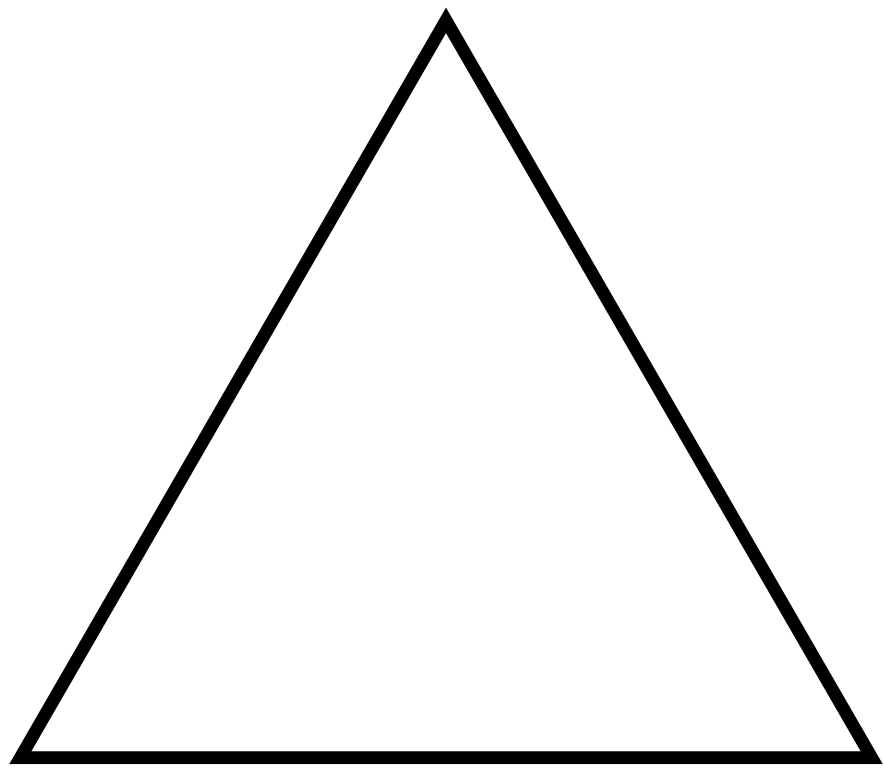
\includegraphics[width=0.5\textwidth]{intro/triangle.png} 
    \end{center}
\end{frame}

\begin{frame}
    \frametitle{Equilateral and Isosceles Triangle}
    \begin{figure}[h]    
        \begin{minipage}[b]{0.4\textwidth}
        \centering
        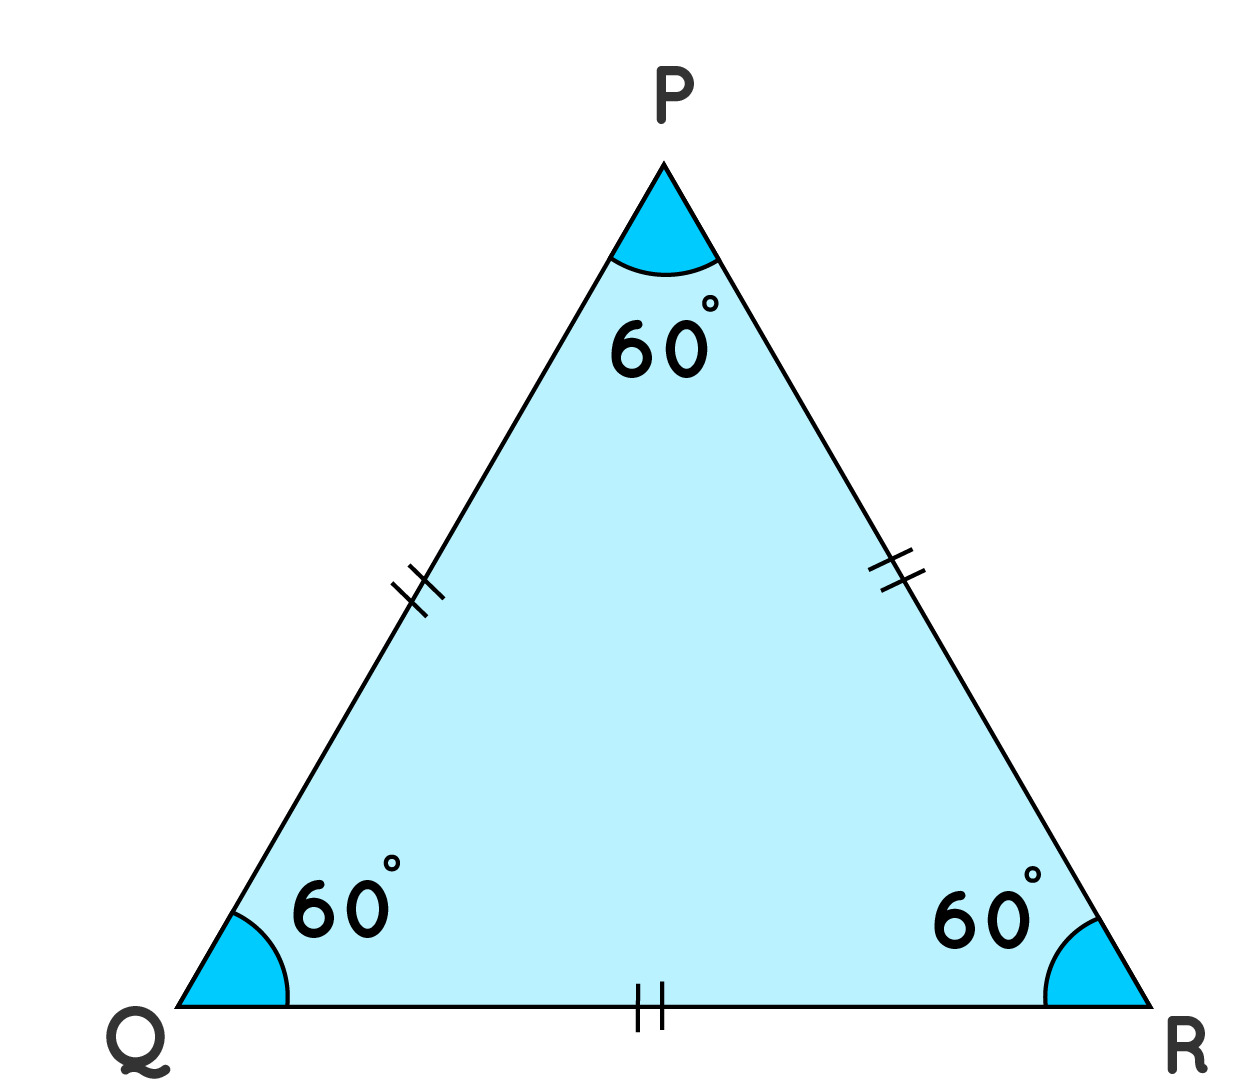
\includegraphics[scale=0.1]{intro/equilateral_triangle.png}
        \caption{Equilateral}
    \end{minipage}
    \begin{minipage}[b]{0.4\textwidth}
        \centering
        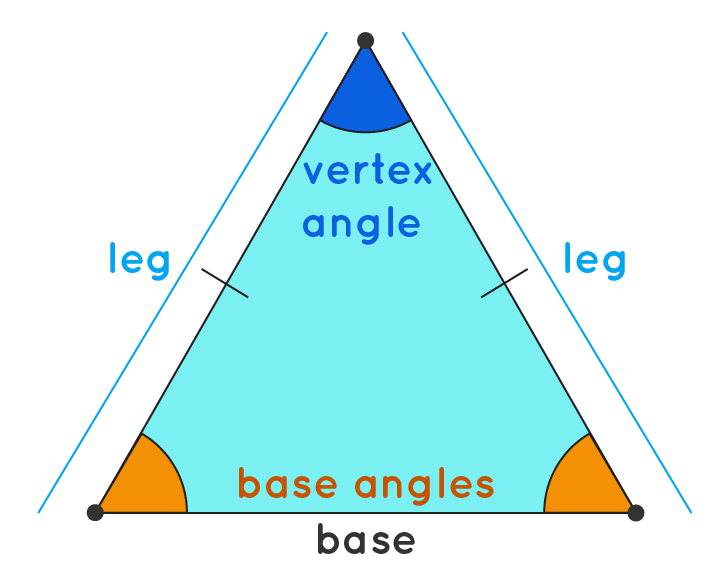
\includegraphics[scale=0.15]{intro/isoscles_triangle.png}
        \caption{Isosceles}
    \end{minipage}
\end{figure}
\end{frame}

\begin{frame}
    \frametitle{Triangle Inequality}
    \begin{block}{}
        For any triangle with sides \(a\), \(b\), and \(c\), the following conditions must hold true:
         \begin{itemize}
                \item \( a + b > c \)
                \item \( a + c > b \)
                \item \( b + c > a \)
        \end{itemize}
    \end{block}
    \begin{center}
        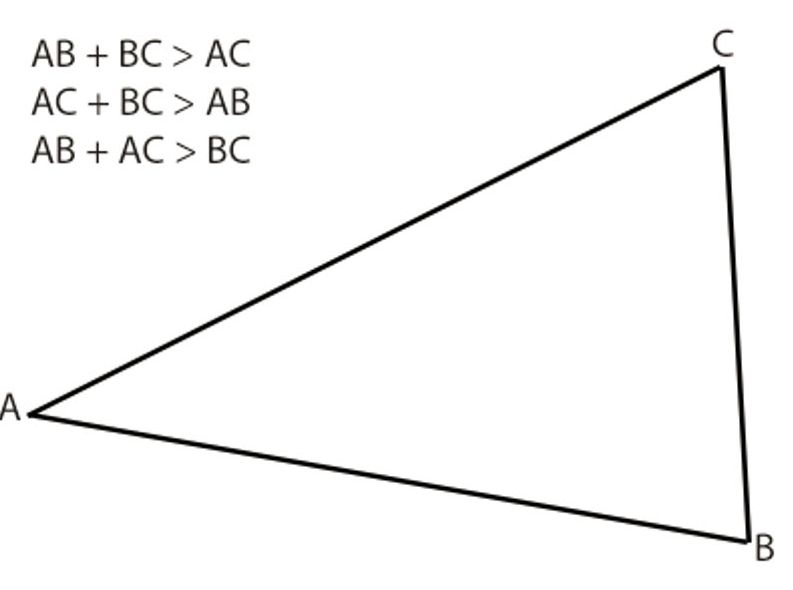
\includegraphics[width=0.3\textwidth]{intro/triangle_inequality.jpeg} 
    \end{center}
\end{frame}

\section{Similarity}

\subsection{Transformations}



    
    % Slide: Introduction
    \begin{frame}{What are Rigid Transformations?}
        \begin{itemize}
            \item Rigid transformations (or isometries) preserve the shape and size of geometric objects.
            \item They do not alter:
            \begin{itemize}
                \item Distances between points.
                \item Angles between lines or curves.
            \end{itemize}
            \item The object remains congruent to itself after the transformation.
        \end{itemize}
    \end{frame}
    
    % Slide: Types of Rigid Transformations
    \begin{frame}{Types of Rigid Transformations}
        \begin{enumerate}
            \item \textbf{Translation:} Moves every point by the same distance in a given direction.
            \item \textbf{Rotation:} Rotates an object around a fixed point by a certain angle.
            \item \textbf{Reflection:} Flips an object over a specified line (the "mirror line").
            \item \textbf{Glide Reflection:} Combines a reflection and a translation along the direction of the reflection line.
        \end{enumerate}
    \end{frame}
    
    % Slide: Translation
    \begin{frame}{Translation}
        \textbf{Definition:}
        \begin{itemize}
            \item Moves every point of an object by the same distance in a specific direction.
        \end{itemize}
        \textbf{Mathematical Representation:}
        \[
        (x', y') = (x + a, y + b)
        \]
        \textbf{Properties:}
        \begin{itemize}
            \item Preserves distances and angles.
            \item Does not change the orientation of the object.
        \end{itemize}
    \end{frame}
    
    % Slide: Rotation
    \begin{frame}{Rotation}
        \textbf{Definition:}
        \begin{itemize}
            \item Rotates an object around a fixed point by a certain angle.
        \end{itemize}
        \textbf{Mathematical Representation:}
        For a rotation by angle \(\theta\) around the origin:
        \[
        x' = x \cos\theta - y \sin\theta
        \]
        \[
        y' = x \sin\theta + y \cos\theta
        \]
        \textbf{Properties:}
        \begin{itemize}
            \item Preserves distances and angles.
            \item Changes the orientation depending on the direction of rotation.
        \end{itemize}
    \end{frame}
    
    % Slide: Reflection
    \begin{frame}{Reflection}
        \textbf{Definition:}
        \begin{itemize}
            \item Flips an object over a line (the "mirror line").
        \end{itemize}
        \textbf{Examples:}
        \begin{itemize}
            \item Reflection across the \(x\)-axis, \(y\)-axis, or any line \(y = mx + c\).
        \end{itemize}
        \textbf{Properties:}
        \begin{itemize}
            \item Preserves distances and angles.
            \item Changes the orientation of the object.
        \end{itemize}
    \end{frame}
    
    % Slide: Properties of Rigid Transformations
    \begin{frame}{Properties of Rigid Transformations}
        \begin{itemize}
            \item \textbf{Distance Preservation:} The distance between any two points remains unchanged.
            \item \textbf{Angle Preservation:} Angles between lines or curves are preserved.
            \item \textbf{Parallelism:} Parallel lines remain parallel.
            \item \textbf{Co-ordinates} Co-ordinates ae not preserved 
            \item \textbf{Congruence:} The original and transformed shapes are congruent.
        \end{itemize}
    \end{frame}
    
  \begin{frame}
    \frametitle{Exercise: Rigid Transformations}
    \begin{center}
        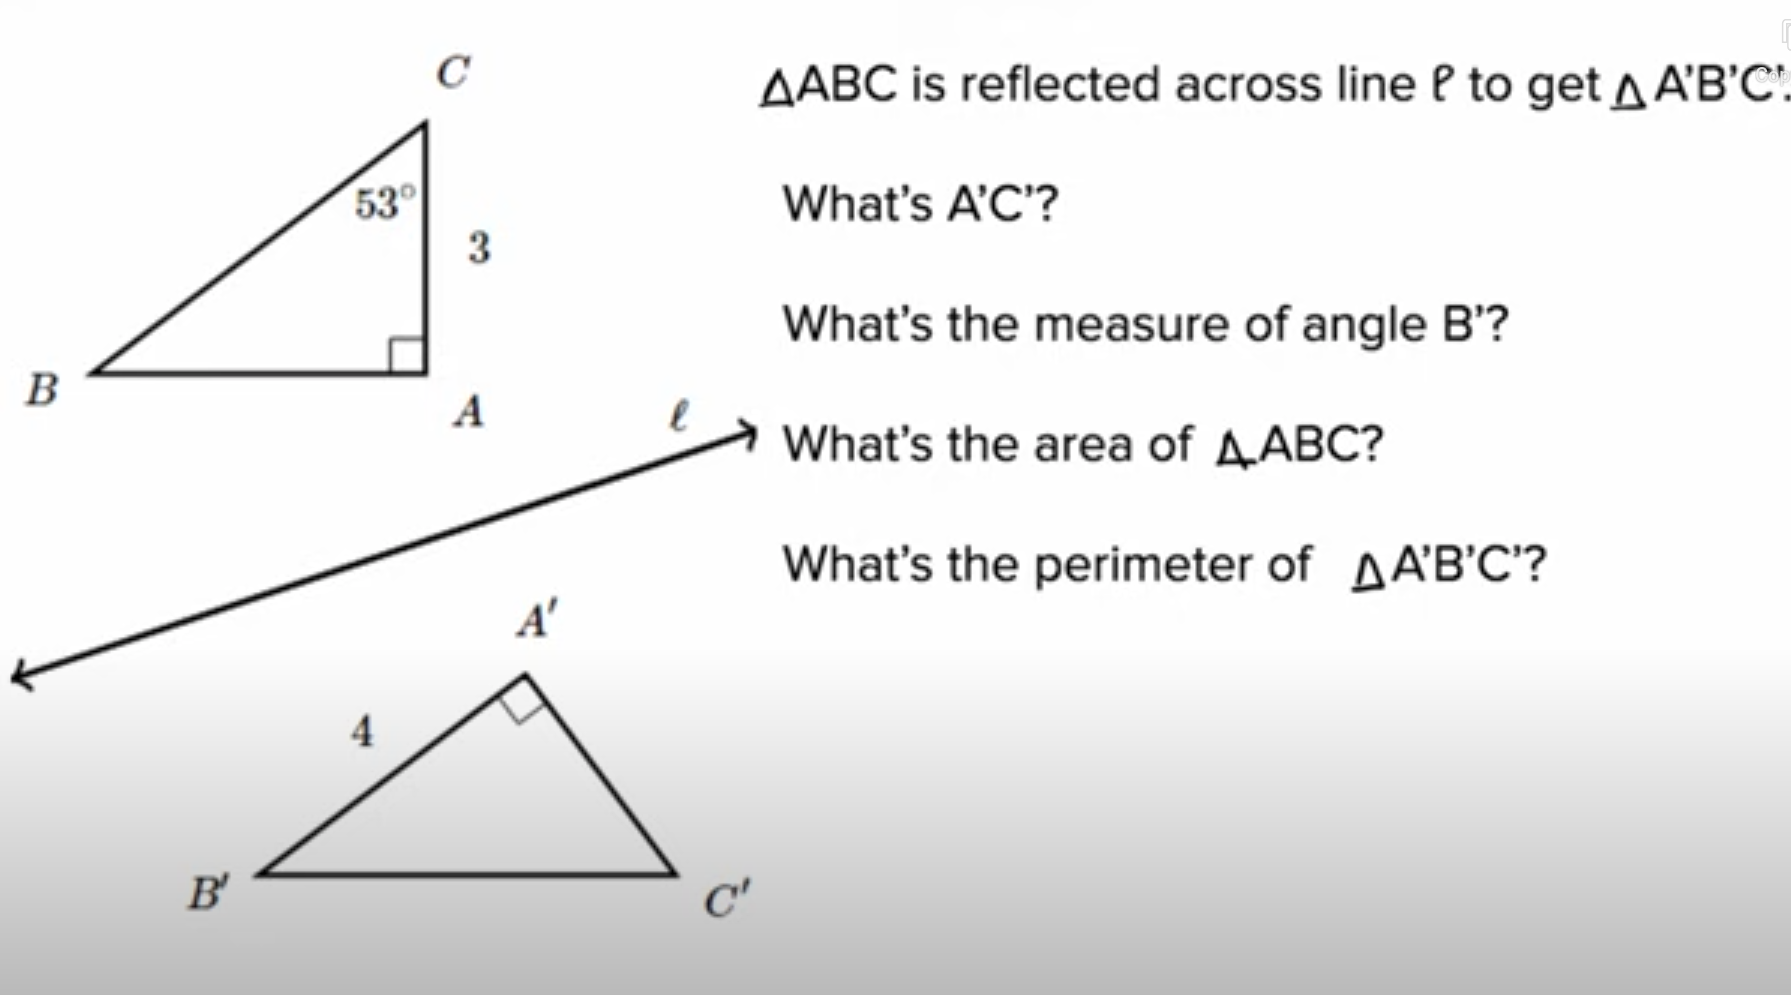
\includegraphics[width=0.9\textwidth]{intro/exer_20.png} 
    \end{center}
  \end{frame}

  \begin{frame}
    \frametitle{Dilations}
    \textbf{Definition:}
        \begin{itemize}
            \item Dilation involves scaling distances from a point (the center of dilation) by a constant factor $k$. It changes the size of a figure but not its shape.
        \end{itemize}
    \begin{itemize}
        \item A non rigid transformation where lengths are not preserved 
        \item Dilation will preserve angles 
    \end{itemize}
\end{frame}
    \subsection{Congruence}
    \begin{frame}
        \frametitle{What is Congruence}
        \begin{block}{Definition}
            Congruence means that two figures or shapes are identical in shape and size. 
            They can be transformed into each other using rigid transformations such as translation, rotation, or reflection 
        \end{block}

        \begin{itemize}
            \item Vertical angles are congruent
            \item Alternate interior angles are congruent
            \item Alternate exterior angles are congruent
            \item Corresponding angles are congruent
        \end{itemize}
    \end{frame}

    \subsection{Congruence in Triangles}
    \begin{frame}
        \frametitle{Congruence in Triangles}
        \begin{block}{SSS}
            if three sides of one triangle are congruent to the three sides of another triangle
        \end{block}
        \begin{block}{SAS}
            if two sides and an included angle of one triangle is congruent to another
        \end{block}
        \begin{block}{ASA}
            if two angles and included side of a triangle is  congruent to another 
        \end{block}
        \begin{block}{AAS}
            if two angles and non included side of a triangle is congruent to another 
        \end{block}
    \end{frame}

     \subsection{Similarity in Triangles}
        \begin{frame}
            \frametitle{Similarity in Triangles}
            \begin{block}{AAA}
                if three angles of one triangle are congruent to another 
            \end{block}
            \begin{block}{SSS}
                if three sides of a triangle are proportional to another
            \end{block}
            \begin{block}{SAS}
                if two sides of a triangle are proportional and included angle is congruent 
            \end{block}
        \end{frame}

\begin{frame}
    \frametitle{What is a Unit Circle}
    \begin{block}{The Unit circle}
        The unit circle is the circle with radius 1 centered at the origin 
    \end{block}
    \begin{block}{Equation of unit Circle}
        The unit circle in the xy-plane is the set of points (x,y) such that
        $$x^{2} + y^{2} = 1$$
        
    \end{block}
    
    \end{frame}
    
    \begin{frame}
    \frametitle{Radius corresponding to a positive angle}
    \centering
    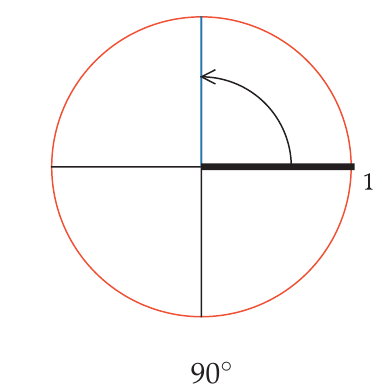
\includegraphics[scale=0.5]{intro/1.png}    \end{frame}
    
    \begin{frame}
    \frametitle{Radius corresponding to a negative angle}
    \centering
    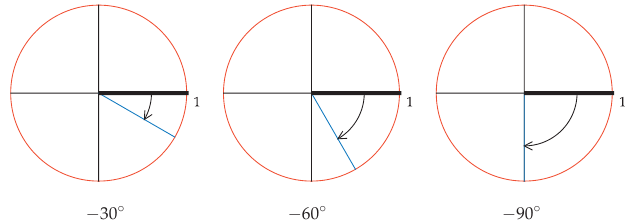
\includegraphics[scale=0.5]{intro/2.png}    \end{frame}
    
    \begin{frame}
        \begin{block}{Positive and Negative Angles}
            \begin{itemize}
                \item Angle measurements for a radius on the unit circle are made from the
                positive horizontal axis.
                \item Positive angles correspond to moving counterclockwise from the positive
                horizontal axis.
                \item Negative angles correspond to moving clockwise from the positive hori-
                zontal axis.
            \end{itemize}
        \end{block}
    \end{frame}
    
    \begin{frame}
        \begin{figure}[h]    
            \begin{minipage}[b]{0.3\textwidth}
            \centering
            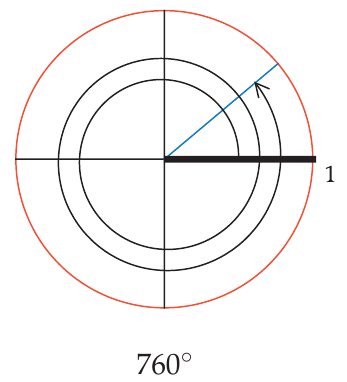
\includegraphics[scale=0.25]{intro/3.png}
            \caption{+ve angle}
        \end{minipage}
        \begin{minipage}[b]{0.3\textwidth}
            \centering
            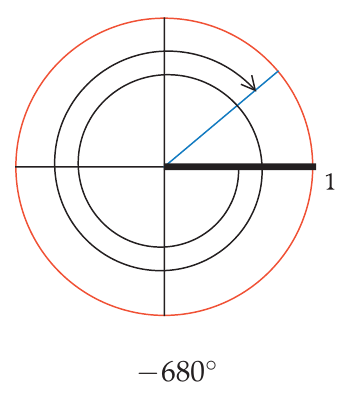
\includegraphics[scale=0.25]{intro/4.png}
            \caption{-ve angle}
        \end{minipage}
    \end{figure}
    \begin{block}{cyclic hehaviour of angles}
        A radius of the unit circle corresponding to $\theta$ degrees also corresponds to
    $\theta + 360n$ degrees for every integer n.
    \end{block}
    \end{frame}
    
    
    \begin{frame}
        \frametitle{Length of a Circular Arc}
        \centering
        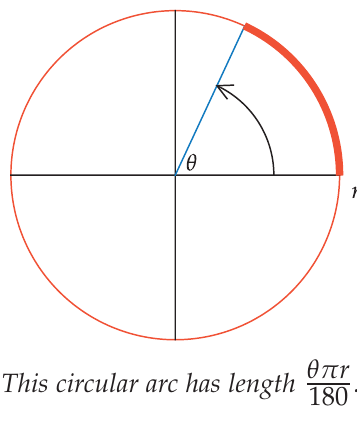
\includegraphics[scale=0.5]{intro/5.png}
    \end{frame}
    
    \begin{frame}
        \frametitle{Radians}
       \begin{block}{Radians}
        Radians are a unit of measurement for angles such that $2\pi$ radians correspond
        to a rotation through an entire circle.
       \end{block}
    \end{frame}
    
    \begin{frame}
        \frametitle{Radians}
        \centering
        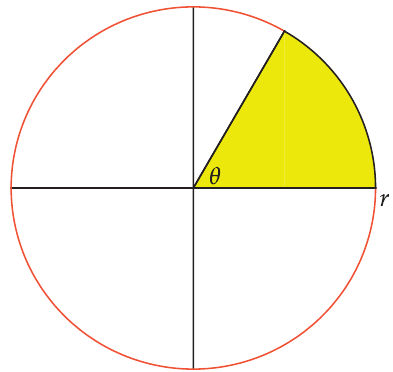
\includegraphics[scale=0.3]{intro/6.png}
    \end{frame}
    \begin{frame}
        \frametitle{Radians}
       \begin{block}{Degree to Radians}
    
        $$ 360^{\circ} = 2 \pi radians $$
        $$ 1 ^{\circ}  = \frac{2 \pi}{360} radians $$
        
       \end{block}
    \end{frame}
    
    \begin{frame}
        \frametitle{Arc Length}
        \begin{block}{length of a circular arc}
            If $0 < \theta \leq 2\pi$ , then a circular arc on the unit circle corresponding to $\theta$ radians
            has length $\theta$         
        \end{block}
    \end{frame}
    
    \begin{frame}
            \begin{figure}[h]    
                \begin{minipage}[b]{0.3\textwidth}
                \centering
                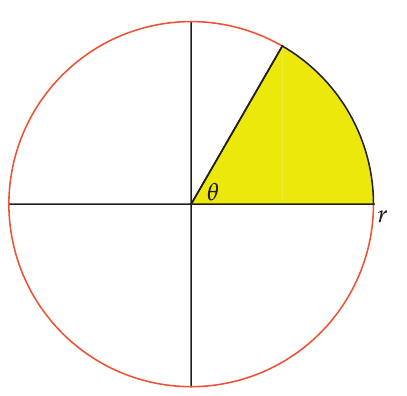
\includegraphics[scale=0.25]{intro/7.png}
                \caption{Area of slice}
            \end{minipage}
        \end{figure}
        \begin{block}{Area of slice}
            A slice with angle $\theta$ radians inside a circle with radius $r$ has area $\frac{1}{2} \theta r^{2}$ .
        \end{block}
    \end{frame}
    
    \begin{frame}
        \frametitle{Cosine and Sine}
        \begin{figure}[h]    
            \begin{minipage}[b]{0.8\textwidth}
            \centering
            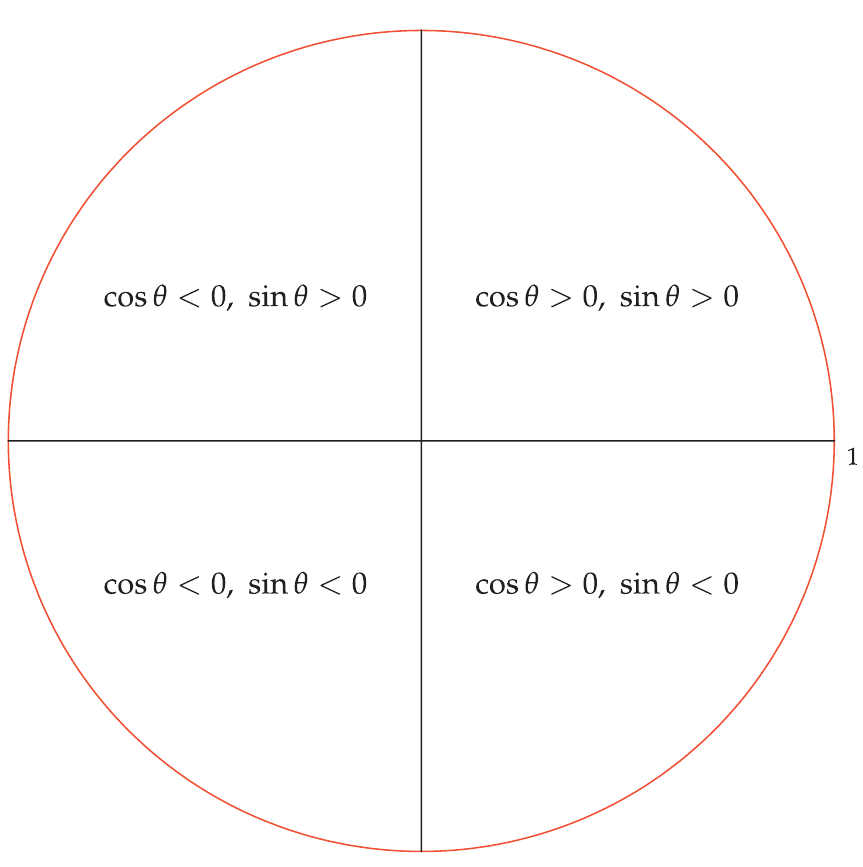
\includegraphics[scale=0.22]{intro/8.png}
            \caption{sin and cos}
        \end{minipage}
    \end{figure}
    \end{frame}


\section{Statistics}
\begin{frame}
    \frametitle{Variability}
    \begin{block}{Variability}
        Variability refers to how data points differ from one another within a data set. In real-world data, there is almost always some variation because no two measurements, observations, or events are exactly the same.
    \end{block}
\end{frame}

\begin{frame}
    \frametitle{Variability Problems}
        \begin{itemize}
            \item How much does my pet weight ?
            \item What is the average number of cars in a parking lot on Monday mornings ?
            \item Am i hungry?
            \item How often am I hungry after lunch ? 
            \item How much time do you spend on facebook every month? 
        \end{itemize}
\end{frame}


\begin{frame}
    \frametitle{Radius corresponding to a positive angle}
    \centering
    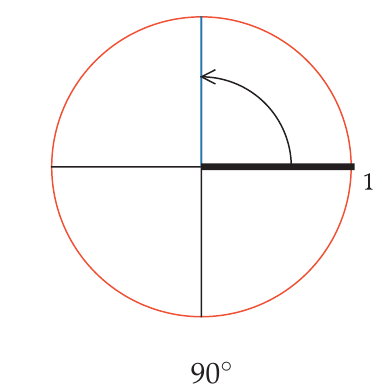
\includegraphics[scale=0.5]{intro/1.png}

\end{frame}

\begin{frame}
    \frametitle{Radius corresponding to a negative angle}
    \centering
    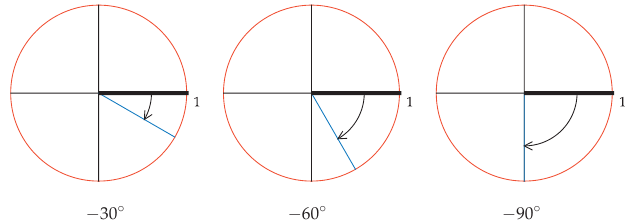
\includegraphics[scale=0.5]{intro/2.png}

\end{frame}

\begin{frame}
    \begin{block}{Positive and Negative Angles}
        \begin{itemize}
            \item Angle measurements for a radius on the unit circle are made from the
            positive horizontal axis.
            \item Positive angles correspond to moving counterclockwise from the positive
            horizontal axis.
            \item Negative angles correspond to moving clockwise from the positive hori-
            zontal axis.
        \end{itemize}
    \end{block}
\end{frame}

\begin{frame}
    \begin{figure}[h]    
        \begin{minipage}[b]{0.3\textwidth}
        \centering
        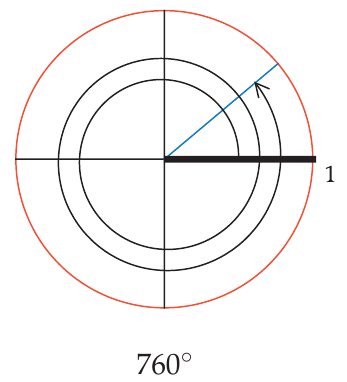
\includegraphics[scale=0.25]{intro/3.png}
        \caption{+ve angle}
    \end{minipage}
    \begin{minipage}[b]{0.3\textwidth}
        \centering
        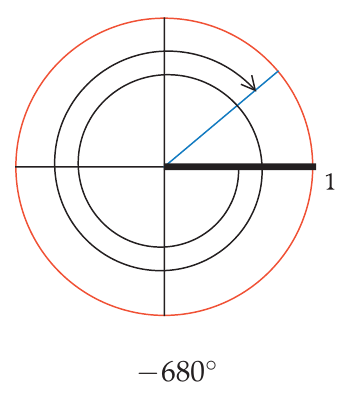
\includegraphics[scale=0.25]{intro/4.png}
        \caption{-ve angle}
    \end{minipage}
\end{figure}
\begin{block}{cyclic hehaviour of angles}
    A radius of the unit circle corresponding to $\theta$ degrees also corresponds to
$\theta + 360n$ degrees for every integer n.
\end{block}
\end{frame}


\begin{frame}
    \frametitle{Length of a Circular Arc}
    \centering
    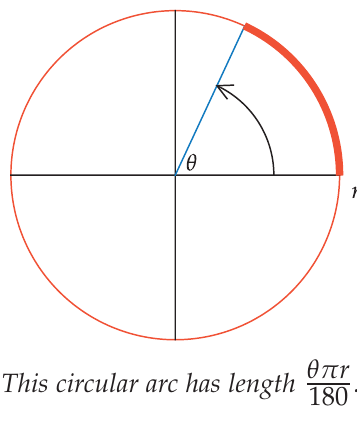
\includegraphics[scale=0.5]{intro/5.png}
\end{frame}

\begin{frame}
    \frametitle{Radians}
   \begin{block}{Radians}
    Radians are a unit of measurement for angles such that $2\pi$ radians correspond
    to a rotation through an entire circle.
   \end{block}
\end{frame}

\begin{frame}
    \frametitle{Radians}
    \centering
    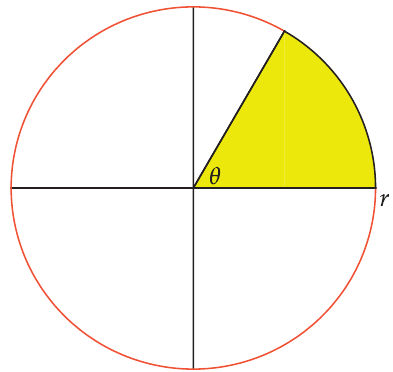
\includegraphics[scale=0.3]{intro/6.png}
\end{frame}
\begin{frame}
    \frametitle{Radians}
   \begin{block}{Degree to Radians}

    $$ 360^{\circ} = 2 \pi radians $$
    $$ 1 ^{\circ}  = \frac{2 \pi}{360} radians $$
    
   \end{block}
\end{frame}

\begin{frame}
    \frametitle{Arc Length}
    \begin{block}{length of a circular arc}
        If $0 < \theta \leq 2\pi$ , then a circular arc on the unit circle corresponding to $\theta$ radians
        has length $\theta$         
    \end{block}
\end{frame}

\begin{frame}
        \begin{figure}[h]    
            \begin{minipage}[b]{0.3\textwidth}
            \centering
            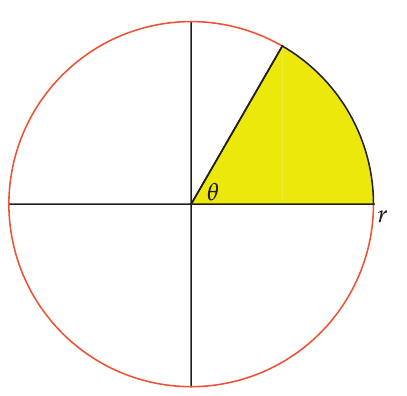
\includegraphics[scale=0.25]{intro/7.png}
            \caption{Area of slice}
        \end{minipage}
    \end{figure}
    \begin{block}{Area of slice}
        A slice with angle $\theta$ radians inside a circle with radius $r$ has area $\frac{1}{2} \theta r^{2}$ .
    \end{block}
\end{frame}
\begin{frame}
    \frametitle{Sine, Cosine and Tangent}
    \begin{figure}[h]    
        \begin{minipage}[b]{0.8\textwidth}
        \centering
        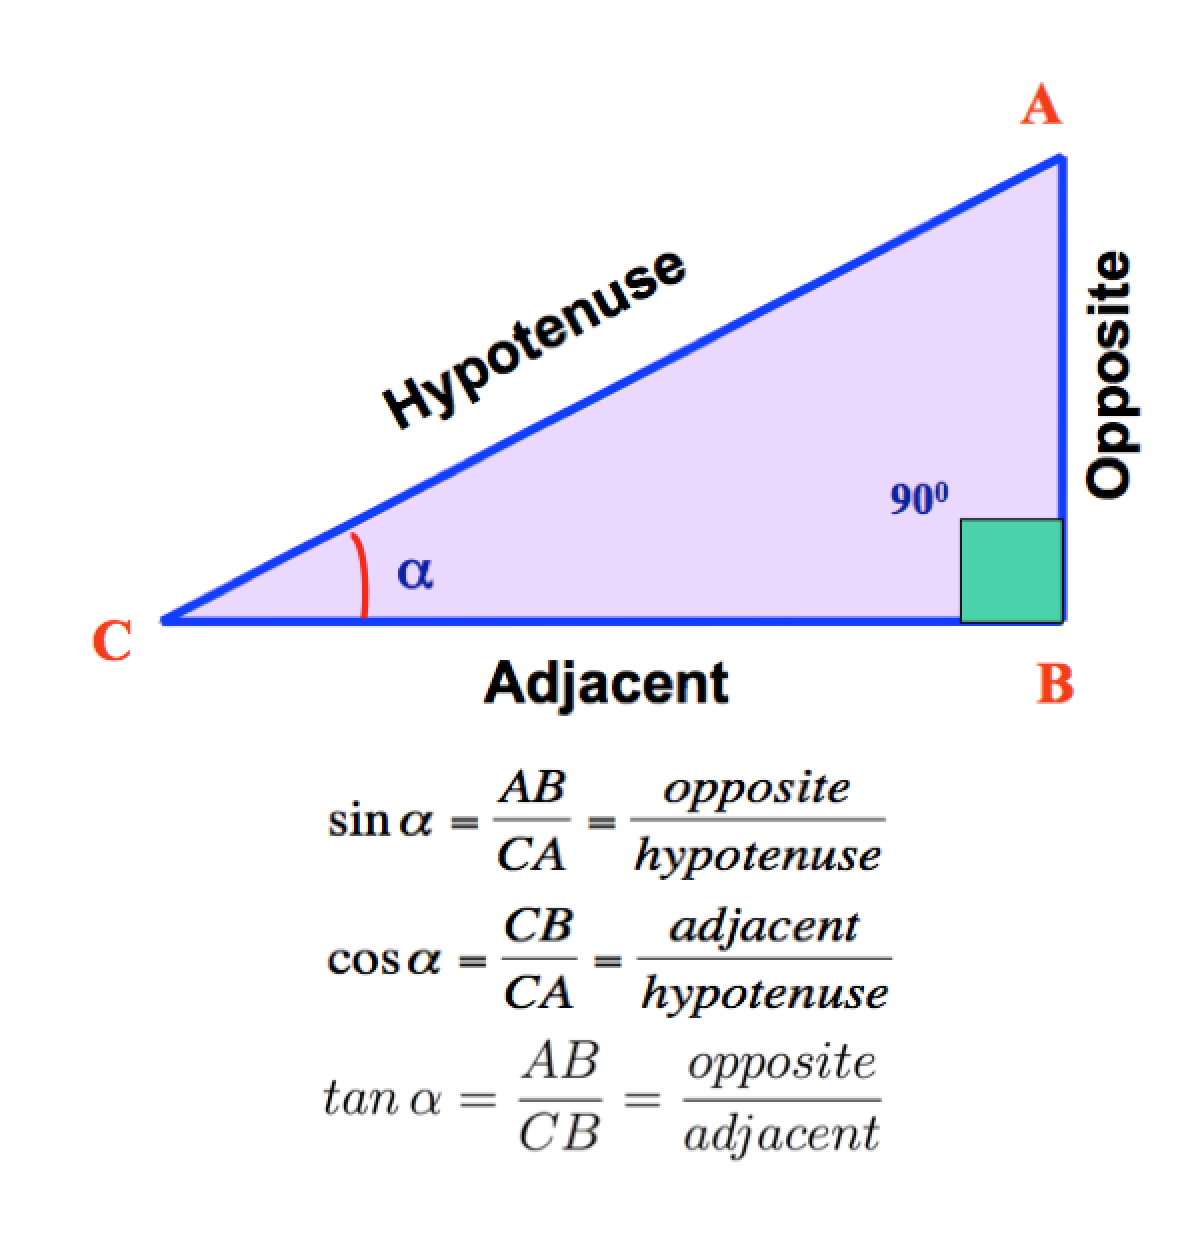
\includegraphics[scale=0.22]{intro/sine-cosine-tangent.png}
    \end{minipage}
\end{figure}
\end{frame}

\begin{frame}
    \frametitle{Unit Circle Co-ordinates}
    \begin{figure}[h]    
        \begin{minipage}[b]{0.8\textwidth}
        \centering
        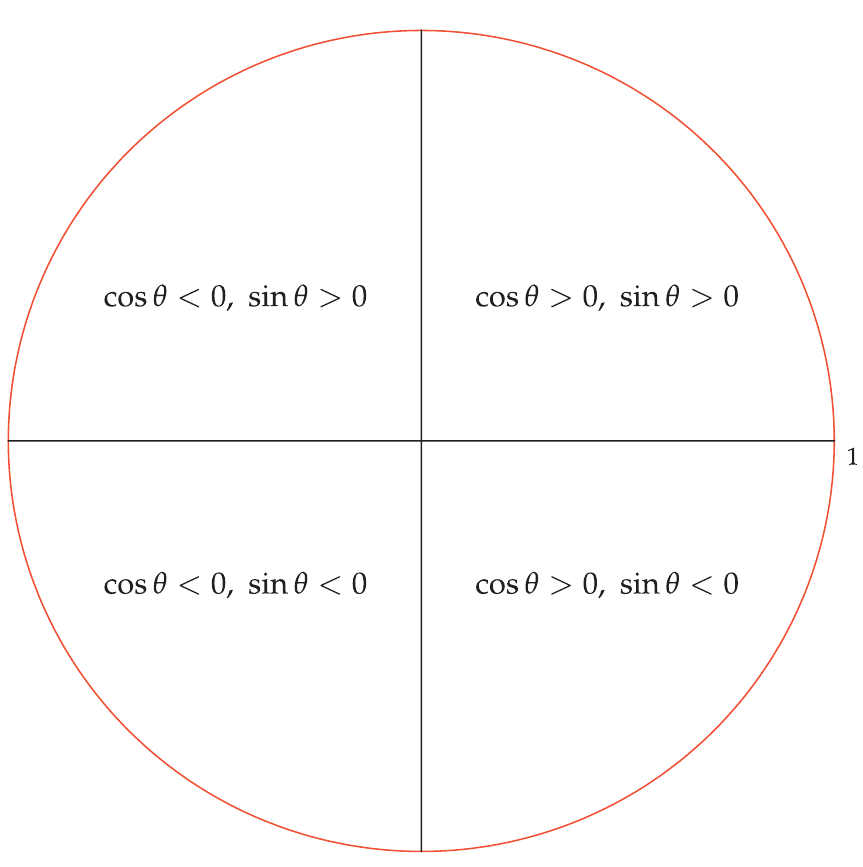
\includegraphics[scale=0.22]{intro/8.png}
    \end{minipage}
\end{figure}
\end{frame}
